\chapter*{Introduction générale}
\markboth{Introduction générale}{Introduction générale}
\addcontentsline{toc}{chapter}{Introduction générale}

Ce rapport porte sur l’étude de méthodes de discrétisation pour la décomposition de Helmholtz--Hodge dans le cas d’une surface fermée sans bord de $\R^3$. On se propose d’adapter des méthodes volumes finis à grilles décalées de type \defini{Discrete Duality Finite Volume} (\ddfv) ayant déjà été employées dans le cas de domaines à bord dans $\R^2$. Cette adaptation nécessite de résoudre des difficultés posées par la géométrie du problème et qui affectent tant l’implémentation numérique des méthodes que l’étude théorique des schémas. \\

Les méthodes \ddfv font partie de la classe des \defini{Volumes Finis à grilles décalées}. Elles reposent sur l'utilisation simultanée de deux maillages duaux l'un de l'autre, généralement appelés maillage \emph{primal} et maillage \emph{dual}. Cette construction permet de définir des opérateurs discrets de gradient et de divergence satisfaisant une propriété de dualité discrète analogue à celle existant au niveau continu. On obtient ainsi une discrétisation des gradients dans toutes les directions de l'espace ce qui permet notamment de se passer des conditions d'admissibilité des maillages souvent associées aux méthodes Volumes Finis. Tout d'abord introduites au début des années 2000 dans des problèmes de diffusion \cite{hermeline_finite_2000}, elles ont dépuis été développées dans d'autres contextes \cite{domelevo_finite_2005,andreianov2009discretedualityfinitevolume,cances_convergence_2010,boyer_ddfv_2017,goudon_ddfv_2019}. Le rapport propose une étude de l'extension de ces méthodes au cas des surfaces fermées de $\R^3$ sans bord. \\

La décomposition de Helmoltz--Hodge est un outil très utilisé et très étudié qui est notamment à la base de la cohomologie de De Rham et qui a des liens étroits avec les équations de Maxwell sous leur formulation potentiel. Elle consiste à décomposer un champ de vecteurs tangents $\vect{u}$ sous la forme :
\[
\vect{u} = \grad \varphi + \grad^\perp \psi + \vect{r}
\]
où $\varphi$ et $\psi$ sont des fonctions scalaires et $\vect{r}$ une fonction vectorielle appartenant au noyau du laplacien (voir la \Cref{fig:dhh}).
\begin{figure}[H]
    \centering
    \def\imgw{0.18\textwidth}
\def\sep{2.1cm}
\def\buf{1.5cm}

\begin{tikzpicture}
\node at (0*\sep,0) {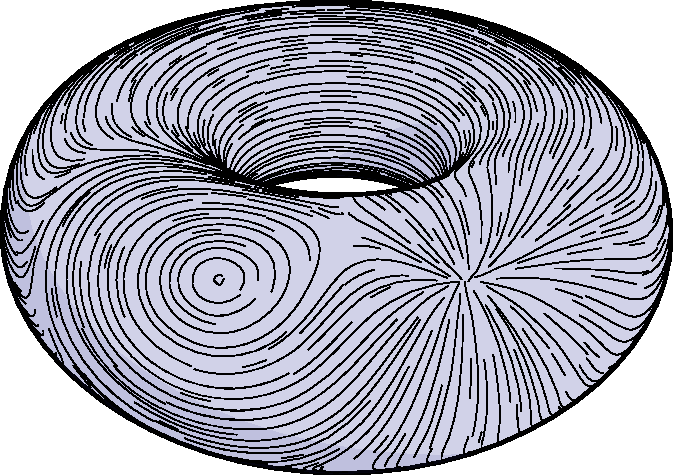
\includegraphics[width=\imgw]{img/input.pdf}};
\node at (1*\sep,0) {\Large $=$};
\node at (2*\sep,0) {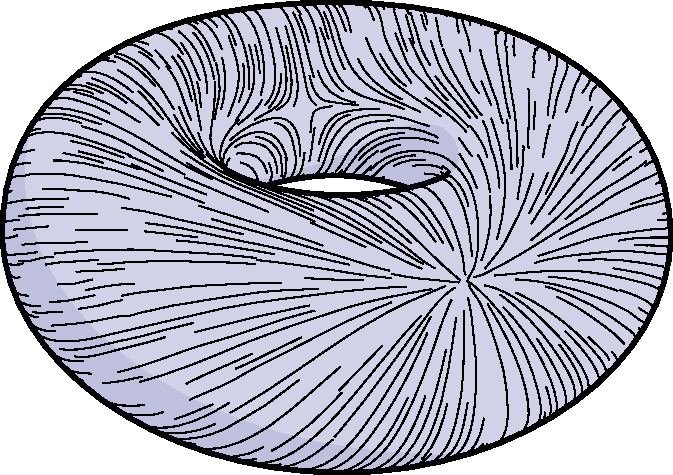
\includegraphics[width=\imgw]{img/grad.pdf}};
\node at (3*\sep,0) {\Large $+$};
\node at (4*\sep,0) {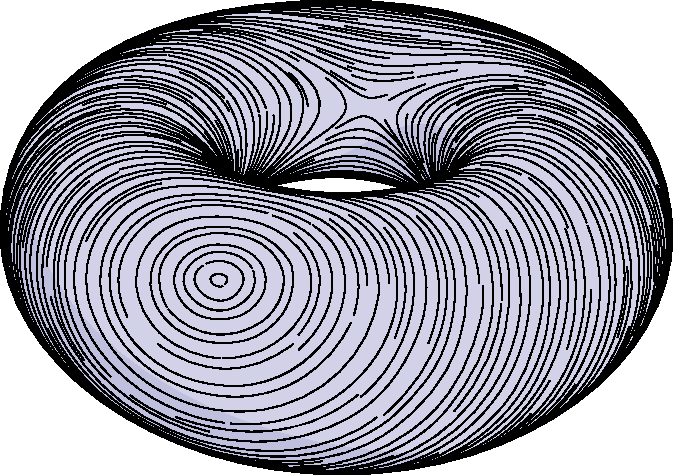
\includegraphics[width=\imgw]{img/rot.pdf}};
\node at (5*\sep,0) {\Large $+$};
\node at (6*\sep,0) {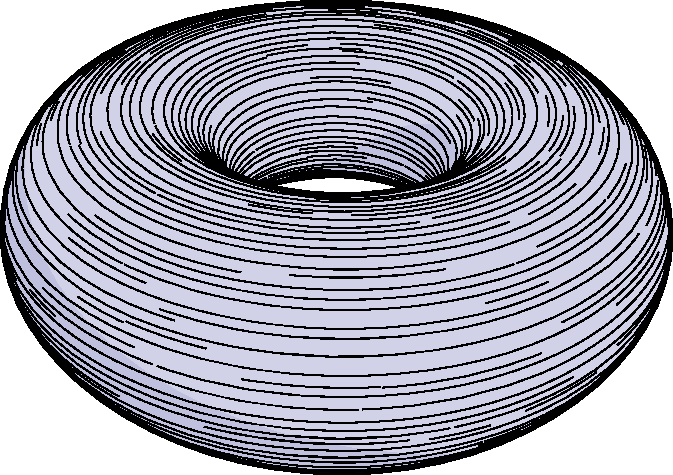
\includegraphics[width=\imgw]{img/harmo.pdf}};

\node at (0*\sep,\buf) {$\vec{u}$};
\node at (2*\sep,\buf) {$\grad \varphi$};
\node at (4*\sep,\buf) {$\grad^\perp \psi$};
\node at (6*\sep,\buf) {$\vec{r}$};
\end{tikzpicture}
    \caption{Exemple de la décomposition de Helmoltz--Hodge sur une surface fermée sans bord de $\R^3$ (crédit K. Crane)}
    \label{fig:dhh}
\end{figure}
Ce problème a déjà été abordé avec succès par des méthodes \ddfv dans le cadre des domaines du plan à bord \cite{delcourte_discrete_2007}. La généralisation des méthodes \ddfv au cadre des surfaces de $\R^3$ sans bord peut se faire en définissant un opérateur de gradient discret dans les plans canoniquement associés aux mailles diamants du maillage et un opérateur de divergence discrète qui soient alors en dualité. Des premiers tests numériques effectués dans le cas simple de la sphère laissent entrevoir une convergence numérique de la méthode et son bon comportement \cite{gregoire_decomposition_2025}. La poursuite de ces tests dans des situations plus critiques présentant notamment une cohomologie non triviale s'accompagnera de l'étude théorique de convergence de la méthode. Les techniques classiques de preuves utilisées en \ddfv reposant sur des résultats de compacité et des inégalités discrètes telles que l'inégalité de Poincaré doivent être adaptées à la géométrie du problème, ce qui concentre en grande partie les difficultés de l'analyse. En effet, l'absence de bord au domaine, permettant généralement de s'assurer de la convergence des solutions primales et duales vers la même solution, ainsi que le fait de se placer dans un cadre de variétés différentielles nécessitent des adaptations aux schémas de preuves classiques et d'établir des estimations discrètes n'existant pas encore dans la littérature pour le cadre \ddfv. \\

Le développement de ces techniques n'en est encore qu'à ses débuts avec relativement peu de travaux présents dans la littérature \cite{tomek_discrete_2016,tomek_discrete_2019} avec des études principalement numériques sans résultats de convergence des méthodes. \\

Les contributions principales de ce rapport sont au nombre de deux et constituent chacune l'objet d'un chapitre. Dans le \textbf{Chapitre I : Généralisation de la méthode \ddfv au cadre des surfaces fermées sans bord de $\R^3$}, nous introduisons un cadre nouveau à cette adaptation de la méthode et définissons la régularité du maillage, les espaces d'approximation, les opérateurs discrets, les produits scalaires et démontrons des propriétés de dualité des opérateurs ainsi qu'une discrétisation de la décomposition de Helmholtz--Hodge. La suite naturelle est de démontrer la convergence de la méthode numérique dans ce nouveau cadre. La démonstration de la convergence repose notamment sur une inégalité de Poincaré dont une démonstration utilisant des techniques inédites dans la littérature \ddfv est proposée dans le \textbf{Chapitre~II : Démonstration de l'inégalité de Poincaré \ddfv sur une surface fermée sans bord de $\R^3$}.

\paragraph{Précisions sur la nature des surfaces considérées}
Dans le titre de ce rapport, nous parlons de \chevron{surface fermée}, dans l'ensemble du rapport nous rajoutons la précision \chevron{sans bord}, dans l'énoncé du \Cref{theo:main}, nous supposons que la surface est \chevron{compacte}. Précisons ces différents termes. Selon certaines acceptions, une surface \defini{fermée} est une surface \defini{compacte} et \defini{sans bord}. Selon cette définition, la sphère, le tore et la bouteille de Klein sont des exemples de surfaces fermées. Un disque ou un ruban de Möbius sont des exemples de surfaces qui ne sont pas fermées. Il faut ajouter à cela la notion d'\defini{orientabilité}. L'orientabilité est une propriété des surfaces dans l'espace euclidien qui mesure s'il est possible de faire un choix cohérent de vecteur normal de surface en chaque point. Par exemple, la bouteille de Klein se distingue de la sphère et du tore par son caractère \defini{non orientable}. Nous excluons les surfaces non orientables. Finalement, les seules surfaces que nous considérons sont les surfaces 
\begin{center}
\textbf{compactes}, \textbf{connexes}, \textbf{sans bord} et \textbf{orientables}.
\end{center}
Le théorème de classification des surfaces nous assure que toute surface de cette nature est homéomorphe à la sphère $\mathbb{S}^2$ ou à la somme connexe de $g$ tores ($g \geqslant 1$), illustrés par la \Cref{fig:sphere_et_n-tore}. De plus, une propriété remarquable des surfaces compactes est qu'elles admettent toujours une triangulation par un nombre fini de triangles. Une autre manière de définir ces surfaces est de les définir comme le bord de tout ouvert borné (lisse) de $\R^3$; $\surflisse \defeq \partial \mathcal{O}$ pour $\mathcal{O} \subset \R^3$.

\begin{figure}[H]
\centering
\begin{subfigure}[t]{.5\textwidth}
    \centering
    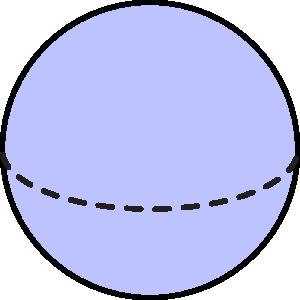
\includegraphics[width=0.2\textwidth]{img/sphere.pdf}
    \caption{Sphère $\mathbb{S}^2$}
\end{subfigure}%
\begin{subfigure}[t]{.5\textwidth}
    \centering
    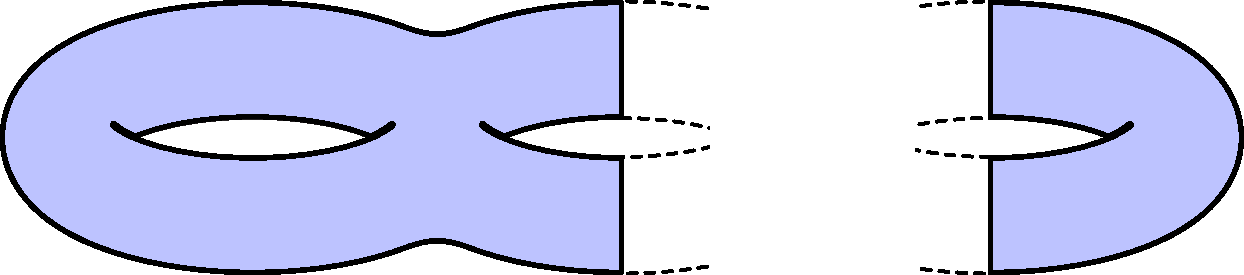
\includegraphics[width=0.8\textwidth]{img/n-tores.pdf}
    \caption{Somme connexe de $g$ tores}
\end{subfigure}
\caption{Surfaces compactes, connexes, sans bord et orientables}
\label{fig:sphere_et_n-tore}
\end{figure}


\begin{comment}
\section{Contexte de la thèse}

\begin{itemize}
    \item Diffraction électromagnétique par un objet
    \begin{figure}
        \centering
        \begin{tikzpicture}[
    scale=1.1,
    every node/.style={font=\footnotesize},
    every path/.append style={line cap=round}
]

\begin{scope}[shift={(0.5,0.25)}]
\draw[myblue, thick, ->] (-4,0) -- (-3,0);
\draw[myblue] (-3.7,-0.4) -- (-3.7,0.4);
\draw[myblue] (-3.5,-0.4) -- (-3.5,0.4) node[above] {onde incidente};
\draw[myblue] (-3.3,-0.4) -- (-3.3,0.4);
\end{scope}

\node[anchor=south west, inner sep=0] (obs) at (0,0) {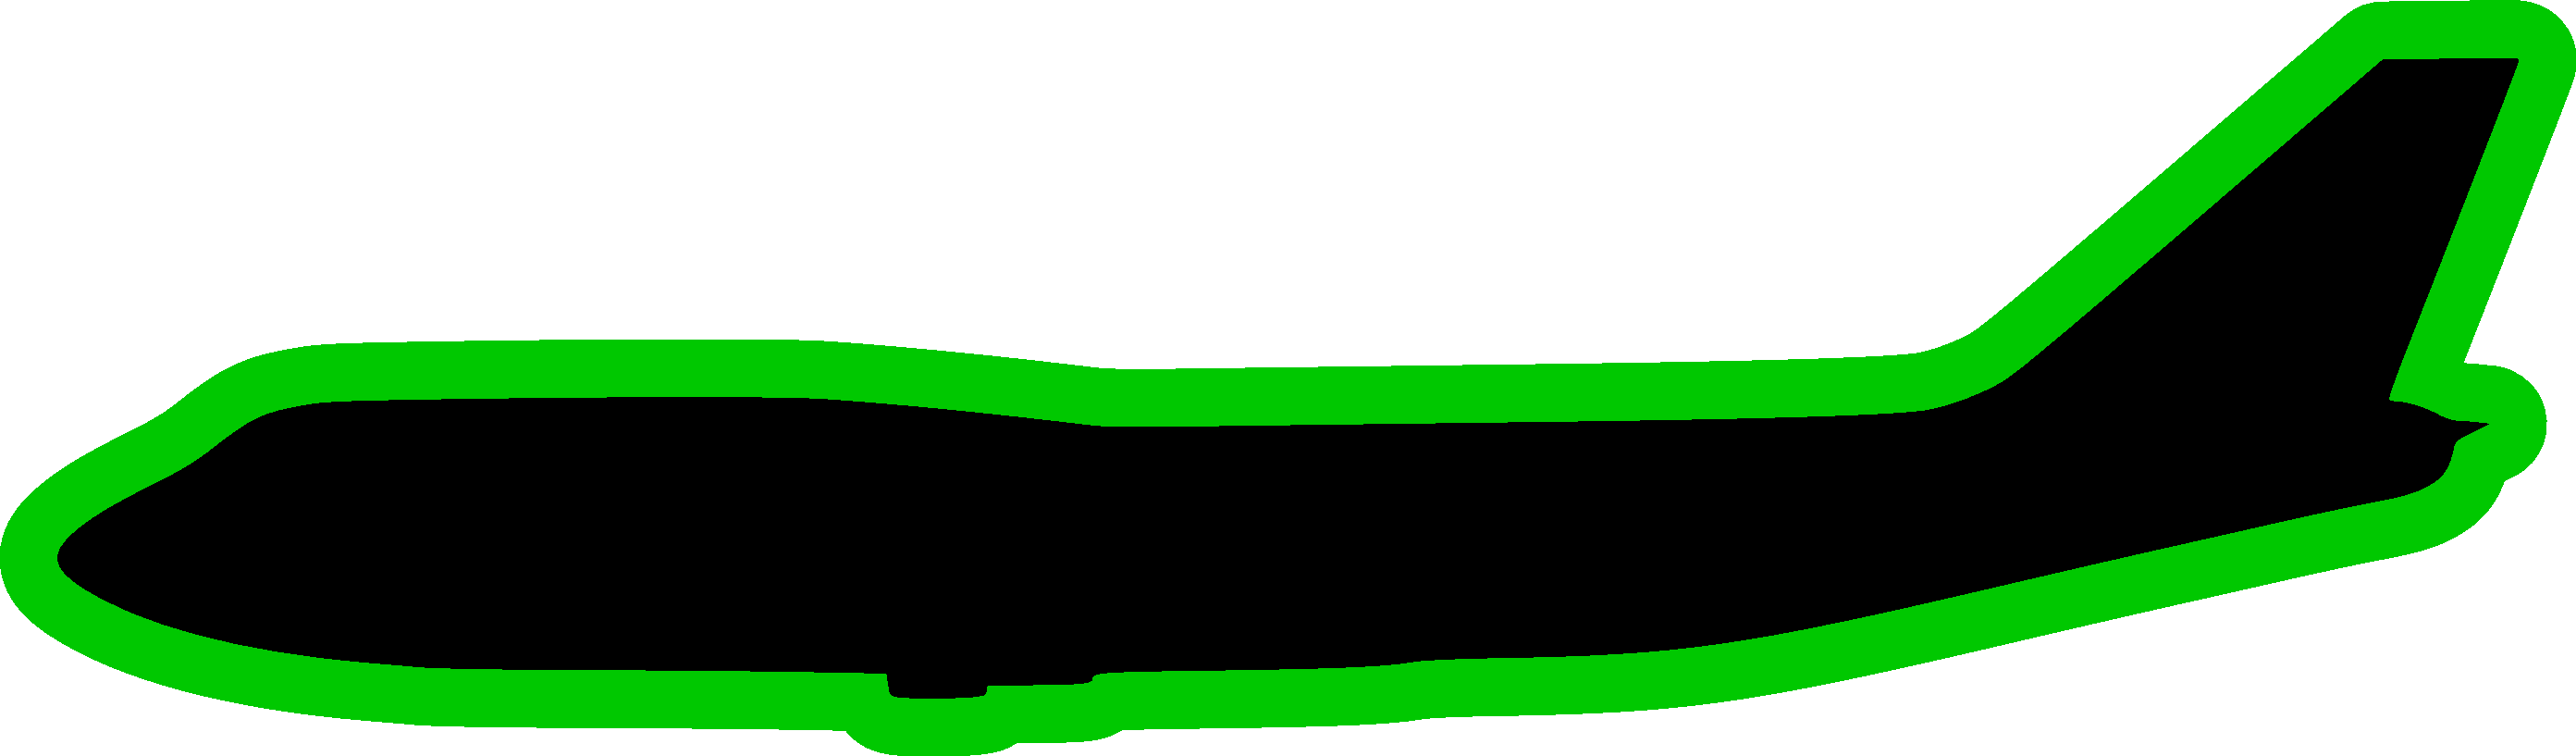
\includegraphics[width=2cm]{img/avion.pdf}};
\node[below=8pt] at (obs.center) {obstacle};
\node[mydarkgreen, right] at (obs.east) {$\Sigma$};

\begin{scope}[rotate=-45, shift={(0.03,0.25)}]
    \draw[decoration={expanding waves, segment length=3mm, angle=40}, decorate, myred] (0, 0) -- ++(-1.2,0) node[right=25pt] {onde diffractée};
    \draw[myred, thick, ->] (-0.2,0) -- (-1.3,0);
    \draw[myred, thick, ->, rotate around={-25:(0,0)}] (-0.2,0) -- (-1.3,0);
    \draw[myred, thick, ->, rotate around={25:(0,0)}] (-0.2,0) -- (-1.3,0);
\end{scope}

\end{tikzpicture}
        \caption{Diffraction d'une onde électromagnétique par un obstacle}
    \end{figure}
    \item Équations de Maxwell en régime harmonique
    \item Méthode des équations intégrales : \emph{Electric Field Integral Equation} (\efie) sur {\color{mydarkgreen}$\Sigma$}
    \[
    \gamma^\mathrm{tan} \mathopen{}\left( \mathrm{i} \, \omega \mu_0 G \vec{J} + \frac{\mathrm{i}}{\omega \varepsilon_0} \grad G \, \mathrm{div} \vec{J} \right) = E^\mathrm{tan}_\mathrm{inc}
    % \gamma^\text{tan} T = \gamma^\text{tan} \left( \mathrm{i}\, \omega \mu_0 G + \frac{\mathrm{i}}{\omega \varepsilon_0} \grad G\, \text{div} \right)
    \]
    \item Matrices \textbf{pleines} et très \textbf{mal conditionnées} % $\implies$ méthodes très lentes
\end{itemize}

\begin{center}
Méthode de \textbf{préconditionnement} : \\
identité de Calder\'on + $\text{div} (n \times \grad \varphi) = 0$ 
\end{center}

\begin{envide}[Conditionnement]
Pour la norme $2$ et $A$ SDP, $\kappa_2(A) = \frac{\lambda_\mathrm{max}(A)}{\lambda_\mathrm{min}(A)}$.
\[
\kappa(A) = \norme{A} \norme{A^{-1}}.
\]
$\div(n \times \grad \varphi) = 0$ ($\varphi$ fonction scalaire sur $\Sigma$) + Calder\'on $\implies$ $\boxed{(n \times T)^2 \approx I + \text{compact}}$
\begin{itemize}
    \item $n \times T$ est bien conditionné
    \item peut servir de préconditionneur
\end{itemize}
\end{envide}

\begin{envide}[\ddfv]
    \begin{itemize}
        \item Conservation des propriétés des opérateurs au niveau discret $\implies$ conserver $\div(n \times \grad \varphi) = 0$ en discret
        \item Permet d'envisager l'inversibilité de la version discrète de l'opérateur $\psi \mapsto n \times \psi$
    \end{itemize}
\end{envide}


\section{Problématique}

\begin{itemize}
    \item L'identité de Calder\'on fournit un moyen élégant de trouver un préconditionneur 
    % une paramétrix de 
    l'opérateur intégral de l'\efie.
    \item Malheureusement, cette identité ne passe pas bien au niveau discret.
\end{itemize}

\begin{envide}[Enjeu principal]
Proposer une méthodologie plus efficace et naturelle via la méthode DDFV
\end{envide}

\begin{envide}[État de l'art]
\begin{itemize}
    \item DDFV pour des domaines à bord dans $\R^2$ (P. Omnes \emph{et al.})
    \item Convergence numérique de la méthode DDFV sur la sphère
    \item Éléments de Whitney sur les surfaces : sans identité de Calder\'on
    \item Éléments finis de Buffa--Christiansen : difficiles à mettre en \oe uvre
\end{itemize}
\end{envide}

\section{Méthode \emph{Discrete Duality Finite Volume} (DDFV)}
\subsection{Classe des méthodes Volumes Finis à \textbf{grilles décalées}}

Discrétisation des gradients dans \textbf{toutes les directions}
Conservation des propriétés des opérateurs au \textbf{niveau discret}

\section{Décomposition de Helmholtz--Hodge}
\subsection{Cas plus simple pour commencer}

\begin{figure}[H]
    \centering
    \def\imgw{0.18\textwidth}
\def\sep{2.1cm}
\def\buf{1.5cm}

\begin{tikzpicture}
\node at (0*\sep,0) {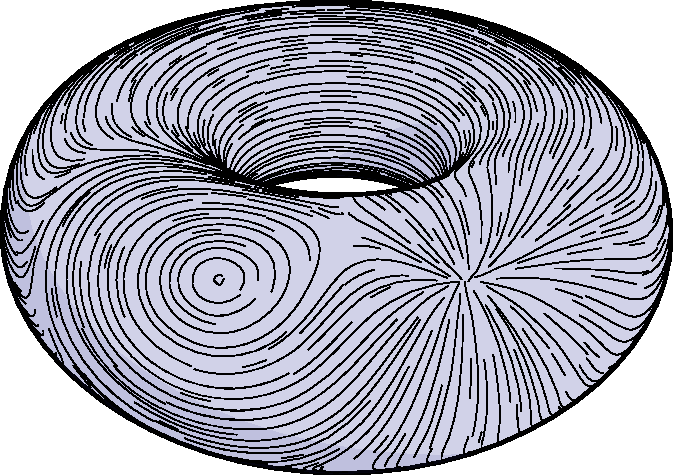
\includegraphics[width=\imgw]{img/input.pdf}};
\node at (1*\sep,0) {\Large $=$};
\node at (2*\sep,0) {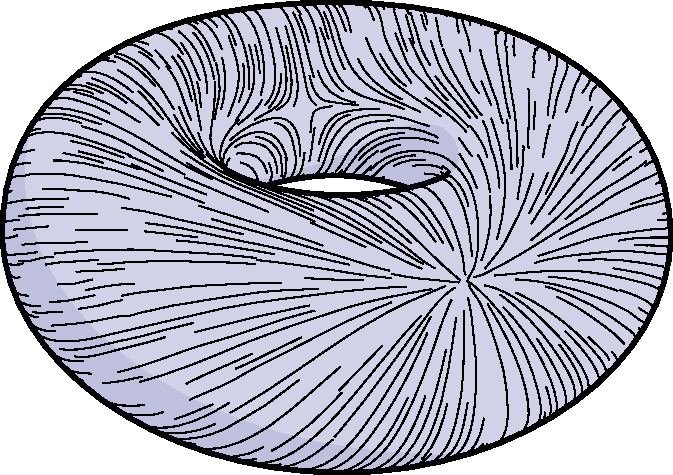
\includegraphics[width=\imgw]{img/grad.pdf}};
\node at (3*\sep,0) {\Large $+$};
\node at (4*\sep,0) {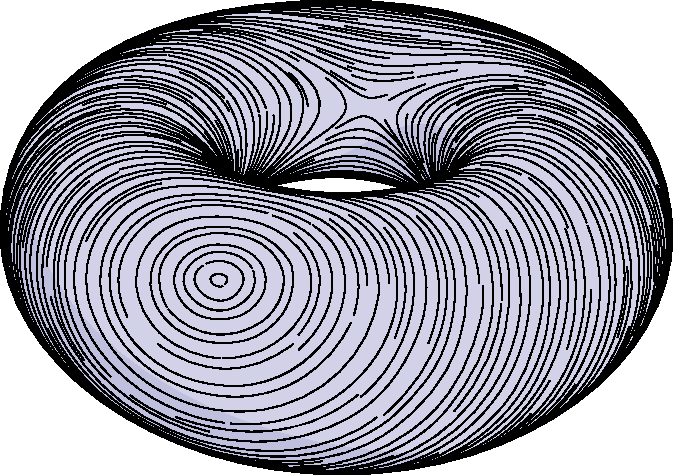
\includegraphics[width=\imgw]{img/rot.pdf}};
\node at (5*\sep,0) {\Large $+$};
\node at (6*\sep,0) {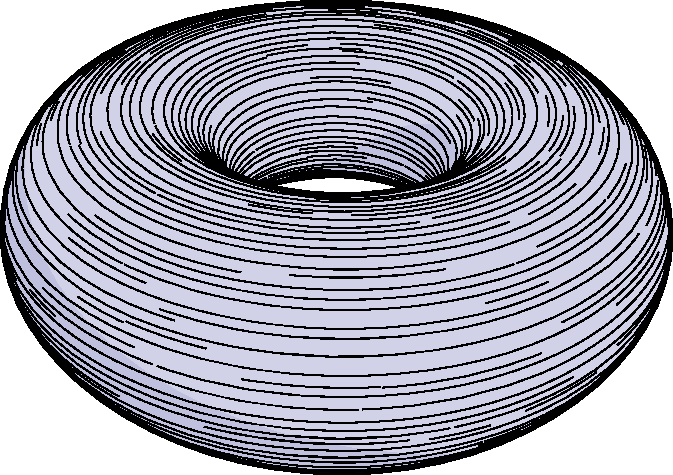
\includegraphics[width=\imgw]{img/harmo.pdf}};

\node at (0*\sep,\buf) {$\vec{u}$};
\node at (2*\sep,\buf) {$\grad \varphi$};
\node at (4*\sep,\buf) {$\grad^\perp \psi$};
\node at (6*\sep,\buf) {$\vec{r}$};
\end{tikzpicture}
    \caption{Exemple sur une surface fermée sans bord de $\R^3$ (crédit Keenan Crane)}
\end{figure}

\begin{remarque}
Un maillage \ddfv est défini de manière unique à partir de $\mathfrak{M} \cup \ens[\big]{x_\mathcal{K} \tq \mathcal{K} \in \mathfrak{M}}$
\end{remarque}

\section{Objectifs de la thèse}

\begin{envide}[Résultats attendus]
\begin{itemize}
    \item Une théorie de l'approximation des champs de vecteurs sur les surfaces de $\R^3$ en DDFV
    \item Une nouvelle méthode de preconditionnement \chevron{à la Calder\'on} de l'\efie
\end{itemize}
\end{envide}

\begin{envide}[Thèmes mathématiques]
\begin{itemize}
    \item Discrétisation par volumes finis
    \item Équations intégrales
    \item Décomposition de Helmholtz--Hodge
    \item Implémentation numérique et preuve de convergence
\end{itemize}
\end{envide}

\begin{envide}[Techniques de preuve]
\begin{itemize}
    \item Adaptation des schémas de preuves classiques au cadre des variétés différentielles 
    \item Résultats de compacité
    \item Inégalités discrètes de type Poincaré adaptées à la géométrie
    \item Lien avec l'homologie
\end{itemize}
\end{envide}
\end{comment}